%\title{shortPaper_TABD}

\documentclass{llncs}

\usepackage[english]{babel}
\usepackage{fontenc}
\usepackage[utf8]{inputenc}
\usepackage[export]{adjustbox}
\usepackage{amsmath}
\usepackage{graphicx}
\usepackage[colorinlistoftodos]{todonotes}
\usepackage{placeins}
\usepackage{makeidx}
\usepackage{blindtext}
\usepackage{amssymb}
\usepackage{multirow}
\usepackage{indentfirst}

\begin{document}

\title{%
The Big \textit{Boom} of \textit{Big Data}  %\textit{Short Paper}
}

\author{%
Ricardo Fusco}

\institute{%
  Universidade de Évora, Portugal \\
  \email{ricardo.fusco2@gmail.com}
 }

\date{}


\maketitle{}

\begin{abstract}
Nowadays we find ourselves in the golden age of \textit{Big Data} with this concept being a rising trend. Given the exponential rise in the amount of data being generated daily by all kinds of companies, it was inevitable to stumble upon a whole new array of markets with the capture and analysis of all types of data in order to provide a full picture of most of the business related aspects and adapt to the ever changing needs and behavior of costumers. Along with all the new technologies available to deal with large volumes of data came \textit{Data Warehousing} and \textit{Business Intelligence}~\cite{Chen2012} completely revolutionizing the IT industry.

\end{abstract}

\section{Introduction}
A few years ago it was almost unthinkable to try dealing with big amounts of data due to the limitations regarding storage and CPU technologies reaching the point where scalability became a serious problem. Then came along Moore's law tipping the scales for the IT industry resulting in the development of more efficient, effective, robust and faster storage and CPU technologies. This law basically states that the processing power/capacity and processing speeds, more specifically the number of transistors in the processor, double every two years ~\cite{mooreslaw}~\cite{Shaw2014}~\cite{Russom2011}. 

\FloatBarrier
\begin{figure}[ht!]
\centering
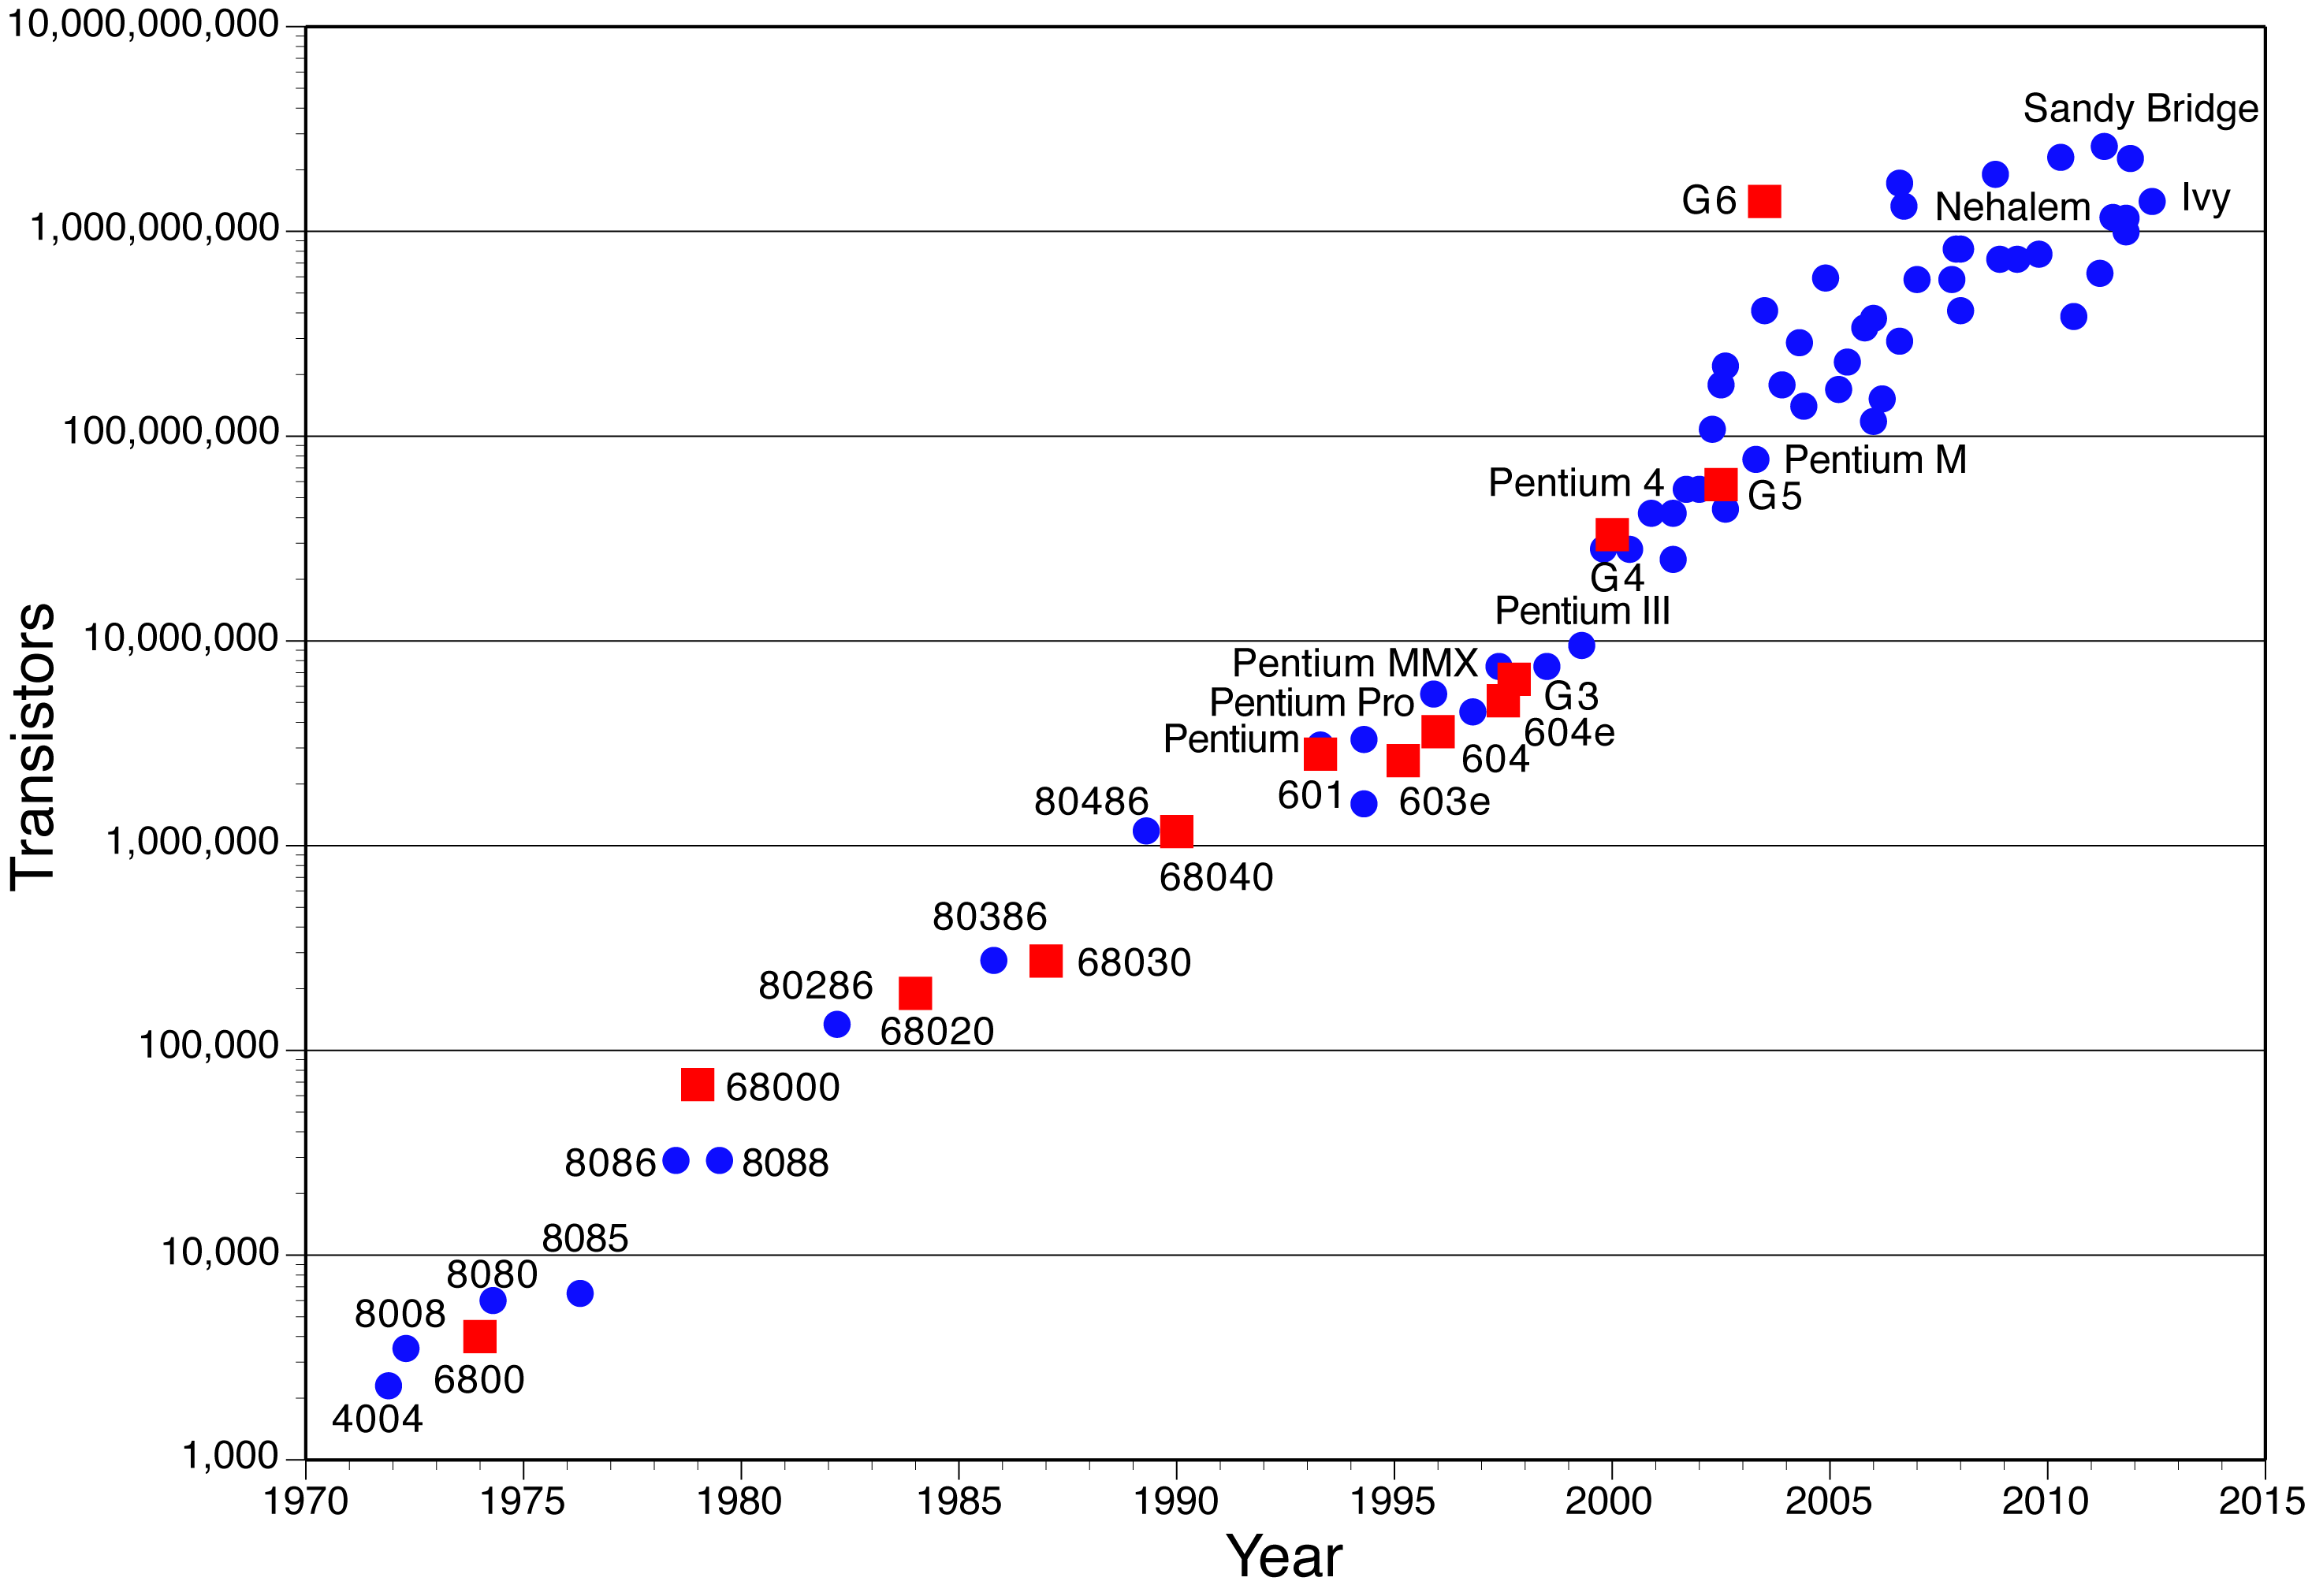
\includegraphics[scale=0.31]{Moores_Law.png}
\caption{Moore's Law~\cite{mooreslawgraph}}
\label{fig:minipage1}
\end{figure}
\FloatBarrier


This all lead to today where companies seek new and inexpensive ways to acquire and analyze data in order to gather facts, new information, basically data about the data per se. What is being revolutionary in the \textit{Big Data} era is not so much the enormous amounts of data being generated but what one can do with it. Furthermore, with the amount of technologies and tools now available and still being created, it is now possible to more efficiently and effectively address the needs of the costumers and improve the user experience.~\cite{Shaw2014}

\section{Big Data}

The \textit{Big Data} phenomenon is mostly due to the continuous advances being made in technology allowing for a deeper understanding of everything and of the best courses of action to take regarding the discovered facts. The pace at which the data is being generated keeps growing at an astounding rate every single day. And it is not merely just about the increasing quantities of data but also about the new types of data being created, like, for instance, data gathered by all kinds of sensors. ~\cite{Kelly2013}~\cite{Russom2011}

\begin{figure}[ht!]
\centering
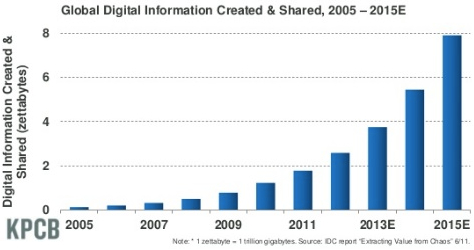
\includegraphics[scale=0.65]{Digital_content_created.jpg}
\caption{Digital content generated and shared per year (zettabytes)~\cite{digitalInfo}}
\label{fig:minipage1}
\end{figure}

Data availability is less and less an issue, most of which is random bits and pieces of meaningless data which must be properly processed in order to make some sense out of it. All of this adds up to the \textit{Big Data} revolution. Things like business intelligence, artificial intelligence techniques like machine learning, pattern recognition can greatly benefit from this accelerating furthermore the evolution in computational techniques.\\

But it is not all a bed of roses. As \textit{Rumpelstiltskin}, the dark one, is used to saying - "All magic comes with a price." - the same applies to \textit{Big Data}, it also has its downsides and negative aspects. When working with massive amounts of data, doing thorough analysis of these data, statistics and other kinds of data analysis the risk of reaching wrong or meaningless conclusions is quite considerable, like looking for a small needle in a colossal haystack of data, misleading and leading one to the inevitable fact here that there are “many bits of straw that look like needles”.~\cite{Boyd2012}

Another crucial negative point regarding \textit{Big Data} is the ethical consequences associated with the privacy issues, studies on some sets of data can harm and/or breach one's privacy which can sometimes lead to another problem which is the uncertainty related with the amount of damage one might or might inflict upon someone while using data sets about humans, not only that but there are also "Numerous companies that collect and sell, consumer profiles that are not clearly protected under current legal frameworks,...”~\cite{Boyd2012} resulting sometimes in illegal, or less legal, brokerage of data regarding subjects. Breaches of data can be equally damaging to one's privacy, for example, breaches to someone's medical records, social records, etc. The progress and developments made in the future regarding the privacy/anonymity issue remain to be seen.~\cite{Boyd2012}~\cite{TaylorArmerding2014}~\cite{Lohr2012}


\section{Fields/areas where \textit{Big Data's} potential is being explored}

Taking as an example social networks like \textit{Facebook}, \textit{Twitter}, \textit{Flickr}, \textit{Instagram}, amongst others, we can closely observe how the parsing, processing and measurement of the billions of billions of data generated by these entities can provide information about its users like behavior patterns, potential marketing material and information on how people are connected to each other in an extremely detailed way.~\cite{Lohr2012}

\begin{figure}[ht!]
\centering
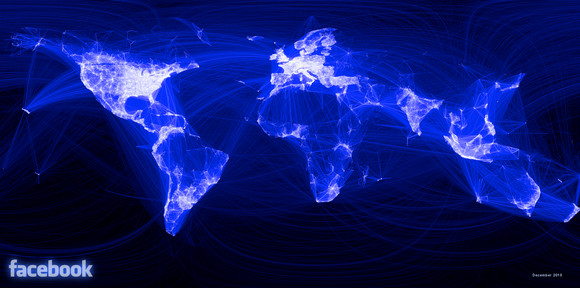
\includegraphics[scale=0.77]{facebook_visualised.jpg}
\caption{Facebook’s global relationships visualized in a global map~\cite{facebookRel}}
\label{fig:minipage1}
\end{figure}

\newpage

In the economic sector it is more and more frequent to see decisions relying on the results provided by the data analysis more so than on experience or induction. Big-box stores and retailers can now thoroughly analyze their prices, successful and unsuccessful sales, and other kinds of data about their costumers.~\cite{Lohr2012}\\

Another clear example of how this \textit{Big Data} trend has been evolving is the oncology sector, with the lowering cost of gene sequencing and the development of the industry making gene sequencing easier, genomic data seems to be getting more and more bountiful and turning gradually more crucial to the development and application of cancer treatments. Clinical organizations and biotechnology companies generate large quantities of genomic data through their research, and quite a lot of organizations have developed initiatives for generating and sharing genomic data from cancer patients and cell lines with the public, which can then be processed and parsed using a \textit{data warehouse} given the need here for data management.~\cite{Tressider2014}~\cite{Lohr2012}

%\newpage

\begin{figure}[ht!]
\centering
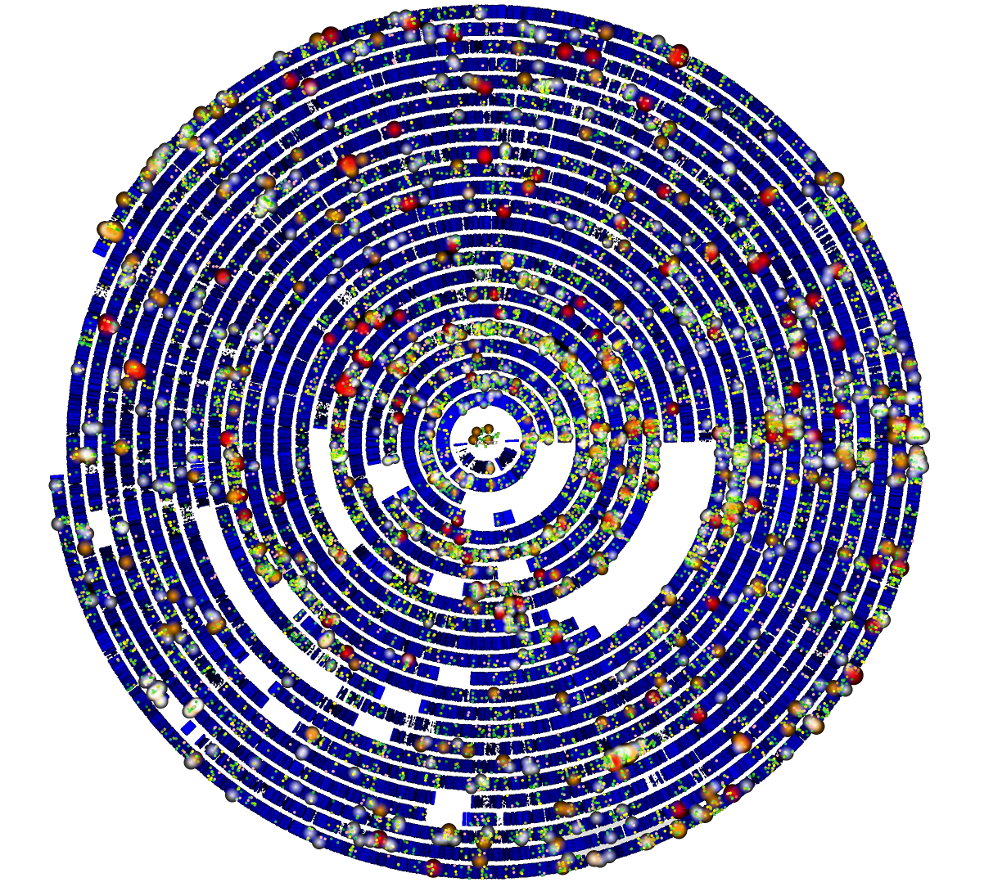
\includegraphics[scale=0.3]{genomic_data.png}
\caption{Genomic data ("Everybody’s uniqueness"). Image by Beat Wolf, Pierre Kuonen and Thomas Dandekar ~\cite{Tressider2014}}
\label{fig:minipage1}
\end{figure}


\section{\textit{Big Data} Technologies}

Nowadays most companies try to turn to the more cheap and efficient technologies in order to treat and make something out of the gathered data, more specifically NoSQL solutions. Why? Well because NoSQL is one of the base groups of \textit{Big Data} technologies, a new and more adequate solution for solving problems that the regular relational database management systems (SQL) seem to have regarding these large amounts of data, like scalability, NoSQL technologies were specially made to be easily scalable thus being cheaper and easier to work with unlike relational databases which are much more complex and costly in terms of servers, licences, extended periods of time for updating and providing new services, etc. Relational databases also have problems dealing with some of the most common data types in these cases like, for example, "unstructured data, blobs of text, sensor data ...".~\cite{Hirleman2014}~\cite{Kelly2013}~\cite{Dix2014}\\ 

One of the several examples of a successful investor in NoSQL technologies is Netflix going from just another boring DVD rental company to one that streams daunting amounts of popular content to millions of viewers generating trillions of transactions per day.~\cite{Hirleman2014}\\ 

If the company seeking for \textit{Big Data} technologies happens to have quite deep pockets then it can, for instance, spend its money on an expensive \textit{Big Data} solution from IBM like some of the largest companies did, like the well known retailer Barnes \& Noble, like Barclays, Mc Donalds UK, within Portugal, Banco Espirito Santo (now named Novo Banco), amongst others.~\cite{IBMcases}~\cite{Hirleman2014}~\cite{Dix2014}~\cite{Oliver2014}\\

Besides NoSQL, Hadoop seems to be a quite valid tool for \textit{Big Data}. This technology is a software framework created in order to "help users handle compute-intensive processes on server clusters with large data volumes. With the help of Hadoop, applications can distribute complex computing tasks across thousands of nodes and process data volumes in the petabyte range ..."~\cite{Konrad} proving to be an essential tool along with NoSQL for accessing and interacting with substantial amounts of data. ~\cite{IBMHad}~\cite{Kelly2013}~\cite{Oliver2014}~\cite{Mitchell2014}~\cite{Lo}~\cite{Russom2011}



\section{Conclusion}

\textit{Big Data} does not comprehend only the data volume, its size whilst in storage, it goes beyond that encompassing also two more properties, speed at which data is processed and data types' diversity. ~\cite{Russom2011}

There are lots of sectors/areas which benefit greatly from the data analysis, using data warehouses and applying Business Intelligence techniques to further improve one's business. There are also the downsides to this trend, which will be interesting to see how it plays out.
The \textit{Big Data} topic however remains a quite "hot" one these days and seems to be an ever growing phenomenon, it brought, and surely is yet to bring, a lot of change and improvement to most of the different sectors/areas. It will be interesting to see how this "boom" of \textit{Big Data} unfolds in the future.   

\bibliographystyle{alpha}
\bibliography{bibliography}

\end{document}